% =====================================================================
%  Diapositivas: Mockito - Grupo 10
%  Compilar:  latexmk -pdf diapositivas.tex
% =====================================================================
\documentclass[aspectratio=169,10pt]{beamer}

\usepackage[T1]{fontenc}
\usepackage[utf8]{inputenc}
\usepackage[spanish,es-tabla,es-noshorthands]{babel}
\usepackage[sfdefault]{FiraSans}
\usepackage[scale=0.85]{FiraMono}
\usepackage{booktabs,tabularx,array}
\usepackage{graphicx}
\usepackage{amssymb}
\usepackage{listings}
\usepackage{tikz}
\usetikzlibrary{arrows.meta,positioning,shapes.multipart,fit,calc,backgrounds,babel}
\usepackage{fontawesome5}
\usepackage[most]{tcolorbox}

\usetheme[progressbar=frametitle,numbering=fraction,block=fill,sectionpage=none]{metropolis}

% ---------- Colores --------------------------------------------------
\definecolor{primario}{HTML}{1F4E79}
\definecolor{acento}{HTML}{C0392B}
\definecolor{verde}{HTML}{1E8449}
\definecolor{gris}{HTML}{5D6D7E}
\definecolor{fondocod}{HTML}{F6F8FA}
\definecolor{kw}{HTML}{7D3C98}
\definecolor{str}{HTML}{1E8449}
\definecolor{com}{HTML}{7F8C8D}
\definecolor{anot}{HTML}{B9770E}
\definecolor{azulclaro}{HTML}{D6EAF8}
\definecolor{verdeclaro}{HTML}{D5F5E3}
\definecolor{rojoclaro}{HTML}{FADBD8}
\definecolor{amarilloclaro}{HTML}{FCF3CF}

\setbeamercolor{frametitle}{bg=primario,fg=white}
\setbeamercolor{progress bar}{fg=anot,bg=primario!30}
\setbeamercolor{title separator}{fg=anot}
\setbeamercolor{alerted text}{fg=acento}
\setbeamercolor{example text}{fg=verde}
\setbeamercolor{block title}{bg=primario!15,fg=primario}
\setbeamercolor{block body}{bg=primario!5}
\setbeamercolor{block title alerted}{bg=acento!15,fg=acento}
\setbeamercolor{block body alerted}{bg=acento!5}
\setbeamercolor{block title example}{bg=verde!15,fg=verde}
\setbeamercolor{block body example}{bg=verde!5}

% ---------- Listings --------------------------------------------------
\lstdefinestyle{java}{
  language=Java, basicstyle=\ttfamily\scriptsize,
  keywordstyle=\color{kw}\bfseries, stringstyle=\color{str},
  commentstyle=\color{com}\itshape, morekeywords={record,var},
  emph={[2]Test,Mock,InjectMocks,Spy,Captor,ExtendWith,DisplayName,ParameterizedTest,CsvSource},
  emphstyle={[2]\color{anot}},
  backgroundcolor=\color{fondocod}, frame=l, framerule=2pt, rulecolor=\color{primario},
  xleftmargin=6pt, framexleftmargin=4pt, breaklines=true, showstringspaces=false,
  columns=fullflexible, keepspaces=true, aboveskip=2pt, belowskip=2pt,
  literate={á}{{\'a}}1 {é}{{\'e}}1 {í}{{\'i}}1 {ó}{{\'o}}1 {ú}{{\'u}}1 {ñ}{{\~n}}1
           {→}{{$\rightarrow$}}2 {≥}{{$\geq$}}1 {≤}{{$\leq$}}1 {º}{{\textordmasculine}}1 {¡}{{!`}}1 {¿}{{?`}}1
}
\lstdefinestyle{bash}{language=bash,basicstyle=\ttfamily\scriptsize,backgroundcolor=\color{fondocod},
  frame=l,framerule=2pt,rulecolor=\color{gris},xleftmargin=6pt,framexleftmargin=4pt,columns=fullflexible,
  literate={á}{{\'a}}1 {é}{{\'e}}1 {í}{{\'i}}1 {ó}{{\'o}}1 {ú}{{\'u}}1 {ñ}{{\~n}}1 {✘}{{\textcolor{acento}{\faTimes}}}1 {✔}{{\textcolor{verde}{\faCheck}}}1}
\lstdefinestyle{terminal}{basicstyle=\ttfamily\tiny\color{white},backgroundcolor=\color{black!88},
  frame=single,rulecolor=\color{black!88},framesep=3pt,xleftmargin=3pt,xrightmargin=3pt,columns=fullflexible,keepspaces=true,
  showstringspaces=false,aboveskip=2pt,belowskip=2pt,
  literate={á}{{\'a}}1 {é}{{\'e}}1 {í}{{\'i}}1 {ó}{{\'o}}1 {ú}{{\'u}}1 {ñ}{{\~n}}1
           {✔}{{\textcolor{green!70!white}{\faCheck}}}1 {✘}{{\textcolor{red!70!white}{\faTimes}}}1 {↷}{{\textcolor{yellow!80!white}{$\curvearrowright$}}}1}
\lstset{style=java}

\newcommand{\code}[1]{\texttt{#1}}

\tikzset{
  caja/.style={draw=primario,fill=azulclaro,rounded corners=2pt,thick,align=center,minimum height=0.8cm,font=\footnotesize},
  ext/.style={draw=gris,fill=gray!12,rounded corners=2pt,thick,align=center,minimum height=0.8cm,font=\footnotesize,dashed},
  flecha/.style={-{Stealth[length=2.2mm]},thick,draw=gris},
  nodo/.style={circle,draw=primario,fill=azulclaro,thick,minimum size=5.5mm,inner sep=0pt,font=\scriptsize\bfseries},
  nodod/.style={nodo,fill=amarilloclaro,draw=anot},
  nodof/.style={nodo,fill=rojoclaro,draw=acento},
  capa/.style={draw=#1,fill=#1!12,thick,rounded corners=3pt,minimum width=13.4cm,minimum height=0.78cm},
  comp/.style={font=\tiny,align=center},
  etq/.style={font=\scriptsize\bfseries,anchor=west,text width=2.1cm},
  k/.style={draw=#1,fill=#1!10,thick,rounded corners=2pt,font=\tiny,align=center,minimum height=0.7cm,minimum width=2.1cm},
  lab/.style={font=\tiny,fill=white,inner sep=1pt},
  fase/.style={draw=#1,fill=#1!12,thick,rounded corners=3pt,minimum height=1.55cm,align=center,text width=2.05cm},
}

\title{Mockito}
\subtitle{Dobles de prueba en Java: SRS, SDD y diseño paso a paso de pruebas de caja negra y caja blanca}
\author{\textbf{Grupo 10}\\[2pt]\small Main Rocabado Jairo Gael \quad Banda Tellez Fernando \quad Velasquez Ricaldez Rodrigo}
\institute{Universidad Mayor de San Simón -- Auditoría de Sistemas}
\date{29 de septiembre de 2026 \quad 08:15 -- 08:44}
\titlegraphic{\hfill\begin{tikzpicture}[scale=0.8]
  \node[caja] (t) {\faFlask\ Test};
  \node[caja,right=0.5cm of t,fill=amarilloclaro,draw=anot] (s) {\faCogs\ SUT};
  \node[ext,right=0.5cm of s] (m) {\faUserSecret\ Mock};
  \draw[flecha] (t) -- (s); \draw[flecha] (s) -- (m);
\end{tikzpicture}}

\begin{document}

\maketitle

\begin{frame}{Contenido}
\begin{columns}[T]
\column{0.48\textwidth}
\begin{enumerate}
  \item El problema y los dobles de prueba
  \item Mockito: qué es y cómo se usa
  \item Arquitectura de Mockito
  \item SRS: especificación de requisitos
  \item SDD: diseño para ser probado
\end{enumerate}
\column{0.48\textwidth}
\begin{enumerate}\setcounter{enumi}{5}
  \item Diseño de casos de prueba paso a paso
  \item Caja negra
  \item Caja blanca
  \item Demo: resultados de la ejecución
  \item Conclusiones
\end{enumerate}
\end{columns}
\vspace{0.6cm}
\begin{block}{Sistema de ejemplo}
\small Un \textbf{Servicio de Pedidos} que verifica el stock, calcula descuentos, cobra con un banco y notifica por correo. Lo especificamos (SRS), lo diseñamos (SDD) y lo probamos con Mockito.
\end{block}
\end{frame}

\section{Dobles de prueba y Mockito}


\begin{frame}{El problema y los dobles de prueba}
\begin{columns}[T]
\column{0.44\textwidth}
\centering
\begin{tikzpicture}[node distance=0.25cm and 0.9cm,scale=0.85,transform shape]
  \node[caja,minimum width=2.6cm,minimum height=1cm,fill=amarilloclaro,draw=anot] (sys) {\textbf{PedidoService}\\\scriptsize clase a probar};
  \node[ext,above right=0.05cm and 0.9cm of sys,minimum width=2.4cm] (bd) {\faDatabase\ Base de datos};
  \node[ext,right=0.9cm of sys,minimum width=2.4cm] (banco) {\faUniversity\ Banco};
  \node[ext,below right=0.05cm and 0.9cm of sys,minimum width=2.4cm] (smtp) {\faEnvelope\ Correo};
  \draw[flecha] (sys) -- (bd); \draw[flecha] (sys) -- (banco); \draw[flecha] (sys) -- (smtp);
\end{tikzpicture}

\vspace{0.2cm}
\begin{alertblock}{Con dependencias reales, la prueba\ldots}
\scriptsize es \textbf{lenta}, \textbf{frágil} (si el banco cae, falla), tiene \textbf{efectos reales} (cobra, envía correos) y no puede provocar un ``pago rechazado''.
\end{alertblock}
\column{0.54\textwidth}
\begin{exampleblock}{Solución: dobles de prueba}
\scriptsize Objetos que \textbf{reemplazan} a las dependencias y que el tester \textbf{controla}.
\end{exampleblock}
\scriptsize
\setlength{\tabcolsep}{3pt}
\begin{tabularx}{\linewidth}{@{}lXl@{}}
\toprule
\textbf{Tipo} & \textbf{Qué hace} & \textbf{En Mockito}\\
\midrule
\alert{Stub} & responde lo programado & \code{when()}\\
\alert{Mock} & registra llamadas para verificarlas & \code{verify()}\\
\alert{Spy} & objeto real que se espía & \code{spy(obj)}\\
Dummy / Fake & relleno / versión simplificada & a mano\\
\bottomrule
\end{tabularx}\\[4pt]
\textbf{Estado}: ¿cuál fue el resultado? $\rightarrow$ caja negra. \textbf{Comportamiento}: ¿cómo interactuó? $\rightarrow$ caja blanca.\\[3pt]
\textcolor{primario}{\faInfoCircle} \textbf{No mockeamos la lógica que queremos comprobar}, sino las dependencias externas o colaboradoras: inventario, pagos, notificaciones y persistencia.
\end{columns}
\end{frame}

\begin{frame}{Mockito en la evaluación de software}
\begin{columns}[T]
\column{0.44\textwidth}
\centering
\begin{tikzpicture}[font=\scriptsize,node distance=0.15cm]
  \node[caja,minimum width=4.6cm,fill=verdeclaro,draw=verde] (e) {\textbf{Estática}: revisiones (sin ejecutar)};
  \node[caja,below=of e,minimum width=4.6cm,fill=amarilloclaro,draw=anot] (d) {\textbf{Dinámica}: pruebas (ejecutando)};
  \node[caja,below=0.25cm of d,minimum width=4.6cm,fill=rojoclaro,draw=acento,line width=1.4pt] (u) {\textbf{Prueba de unidad} $\leftarrow$ Mockito};
  \node[caja,below=of u,minimum width=4.6cm] (i) {Integración $\rightarrow$ Sistema $\rightarrow$ Aceptación};
  \draw[flecha] (d) -- (u);
\end{tikzpicture}

\vspace{0.2cm}
\scriptsize \textbf{Verificación} (¿se construyó bien?) $\rightarrow$ pruebas unitarias.\\
\textbf{Validación} (¿es lo que se pidió?) $\rightarrow$ criterios de la SRS.\\
ISO/IEC 25010: \textbf{capacidad para ser probado}.
\column{0.54\textwidth}
\begin{block}{¿Qué es Mockito?}
\scriptsize
\begin{itemize}
  \item Framework \textbf{open source} (MIT) para crear mocks, stubs y spies en Java.
  \item Creado por Szczepan Faber (2008). Es el \textbf{estándar de facto}: viene incluido en Spring Boot.
  \item Filosofía: \emph{primero ejecuta, después verifica}.
  \item Versión usada: \textbf{5.24.0} (Java 11+), con JUnit 6.
\end{itemize}
\end{block}
\begin{block}{Instalación (Maven)}
\scriptsize \code{mockito-core} y \code{mockito-junit-jupiter}, con \code{<scope>test</scope>}.
\end{block}
\end{columns}
\end{frame}

\begin{frame}[fragile]{Cómo se usa: crear, programar, ejecutar y verificar}
\begin{columns}[T]
\column{0.56\textwidth}
\begin{lstlisting}[basicstyle=\ttfamily\fontsize{6.2}{7.4}\selectfont,breaklines=false]
@ExtendWith(MockitoExtension.class)
class PedidoServiceTest {
    @Mock InventarioRepository inventario; // 1. CREAR:
    @Mock PasarelaPago pasarela;           // un mock por
    @Mock Notificador notificador;         // dependencia
    @Mock PedidoRepository repo;
    @Spy  CalculadoraDescuentos calc;      // lógica real
    @InjectMocks PedidoService servicio;   // SUT + mocks

    @Test
    void pedidoAprobado() {
        // 2. PROGRAMAR
        when(inventario.stockDisponible("MON-01")).thenReturn(10);
        when(pasarela.cobrar(anyString(), anyDouble()))
            .thenReturn(ResultadoPago.aprobado("TX-1"));

        // 3. EJECUTAR
        Pedido r = servicio.procesarPedido(pedido, REGULAR);

        // 4. VERIFICAR
        assertEquals(PAGADO, r.getEstado());
        verify(inventario).descontarStock("MON-01", 2);
    }
}
\end{lstlisting}
\column{0.42\textwidth}
\scriptsize
\begin{tabular}{@{}ll@{}}
\toprule
\textbf{API} & \textbf{Uso}\\
\midrule
\code{when().thenReturn()} & programar respuesta\\
\code{thenThrow()} & simular un fallo\\
\code{doThrow().when(m)} & métodos \code{void}\\
\code{verify(m, times(n))} & verificar llamadas\\
\code{never()} & verificar que no se llamó\\
\code{any()}, \code{eq()} & comodines (matchers)\\
\code{ArgumentCaptor} & capturar argumentos\\
\code{spy()}, \code{mockStatic()} & espiar, simular estáticos\\
\bottomrule
\end{tabular}\\[5pt]
\begin{alertblock}{Sin programar, un mock devuelve}
\scriptsize \code{0}, \code{false}, \code{null}, colecciones vacías u \code{Optional.empty()}.
\end{alertblock}
\end{columns}
\end{frame}

\section{Arquitectura}


\begin{frame}{Arquitectura por capas}
\centering
\begin{tikzpicture}[every node/.append style={}]
\tikzset{comp/.style={font=\scriptsize,align=center}}
  \foreach \y/\c/\t/\txt in {
    0/gris/{1. Tu prueba}/{\code{@Test} · \code{when(...)} · \code{verify(...)}},
    -0.95/primario/{2. API pública}/{\code{Mockito} · \code{@Mock} · \code{@InjectMocks} · \code{ArgumentMatchers} · \code{Answer}},
    -1.9/acento/{3. Núcleo interno}/{\code{MockHandler} · \code{MockingProgress} · \code{InvocationContainer} · \code{VerificationMode}},
    -2.85/anot/{4. Plugins}/{\code{MockMaker} (inline / subclass / proxy) · \code{InstantiatorProvider}},
    -3.8/verde/{5. Bibliotecas}/{\textbf{Byte Buddy} (genera bytecode) · \textbf{Objenesis} (crea objetos sin constructor)},
    -4.75/gris/{6. JVM}/{Instrumentation API · Reflexión · \code{ThreadLocal}}} {
    \node[capa=\c] (n) at (0,\y) {};
    \node[etq] at (n.west) {\t};
    \node[comp] at (1.1,\y) {\txt};
  }
  \foreach \y in {-0.47,-1.42,-2.37,-3.32,-4.27} \draw[flecha] (-6.2,\y+0.12) -- (-6.2,\y-0.12);
\end{tikzpicture}

\vspace{0.15cm}
\scriptsize Solo se usa la capa 2 (\code{org.mockito}). La capa 3 (\code{org.mockito.internal}) puede cambiar entre versiones. La capa 4 permite \textbf{reemplazar piezas} sin tocar Mockito.
\end{frame}

\begin{frame}{Arquitectura: qué pasa en \code{when(inv.stockDisponible("P1")).thenReturn(5)}}
\begin{columns}[c]
\column{0.5\textwidth}
\small Java evalúa \textbf{de dentro hacia fuera}:
\begin{enumerate}\scriptsize
  \item \code{inv.stockDisponible("P1")} llega al \code{MockHandler} (``llamada de ensayo'').
  \item Vacía la \textbf{pila de matchers}: está vacía $\Rightarrow$ \code{"P1"} pasa a \code{Equals("P1")}.
  \item Registra la invocación en el \code{InvocationContainer}.
  \item Avisa a \code{MockingProgress}: ``\textbf{esta es la última invocación}''.
  \item No hay stub $\Rightarrow$ devuelve \code{0} (\code{RETURNS\_DEFAULTS}).
  \item \code{when(0)} ignora el \code{0} y \textbf{toma la última invocación} de \code{MockingProgress}.
  \item \code{thenReturn(5)} crea un \code{Returns(5)}, \textbf{borra} la llamada de ensayo y \textbf{inserta el stub al inicio} de la lista.
\end{enumerate}
\column{0.48\textwidth}
\centering
\begin{tikzpicture}[node distance=0.22cm,font=\tiny]
  \node[caja,minimum width=4.4cm,minimum height=0.55cm] (a) {\code{inv.stockDisponible("P1")}};
  \node[caja,below=of a,fill=rojoclaro,draw=acento,minimum width=4.4cm,minimum height=0.55cm] (b) {MockHandler: registra + avisa};
  \node[caja,below=of b,fill=amarilloclaro,draw=anot,minimum width=4.4cm,minimum height=0.55cm] (c) {MockingProgress: última invocación};
  \node[caja,below=of c,minimum width=4.4cm,minimum height=0.55cm] (d) {\code{when(0)} la toma};
  \node[caja,below=of d,fill=verdeclaro,draw=verde,minimum width=4.4cm,minimum height=0.55cm] (e) {\code{thenReturn(5)} $\rightarrow$ stub guardado};
  \foreach \x/\y in {a/b,b/c,c/d,d/e} \draw[flecha] (\x) -- (\y);
\end{tikzpicture}

\vspace{0.2cm}
\begin{exampleblock}{Reglas que se derivan}
\tiny \faCheck\ Si un argumento usa un matcher, \textbf{todos} deben usarlo: \code{cobrar(eq("a"), anyDouble())}.\\
\faCheck\ Los métodos \code{void} se programan con \code{doThrow().when(mock)}.
\end{exampleblock}
\end{columns}
\end{frame}

\section{SRS}


\begin{frame}{SRS -- Especificación de requisitos (IEEE 830 / ISO/IEC/IEEE 29148)}
\begin{columns}[T]
\column{0.4\textwidth}
\small
\textbf{¿Qué debe hacer el sistema?}\\[3pt]
\scriptsize
\begin{enumerate}
  \item Introducción: propósito, alcance, definiciones
  \item Descripción general: funciones, actores, restricciones, suposiciones
  \item Requisitos específicos:
  \begin{itemize}\scriptsize
    \item Interfaces externas IE-01\ldots04 (\textcolor{acento}{$\Rightarrow$ mocks})
    \item Funcionales RF-01\ldots06 con \textbf{criterio de aceptación}
    \item Reglas de negocio RN-01\ldots04
    \item Casos de uso CU-01, CU-02
    \item No funcionales RNF-01\ldots05
  \end{itemize}
  \item Observaciones de la revisión
\end{enumerate}
\vspace{2pt}\textcolor{verde}{\faArrowRight} \textbf{Base de prueba}: cada caso de caja negra nace de una frase de la SRS.
\column{0.58\textwidth}
\scriptsize
\begin{tabularx}{\linewidth}{@{}lX@{}}
\toprule
\textbf{ID} & \textbf{Requisito}\\
\midrule
RF-01 & Rechazar pedidos sin productos\\
RF-02 & Verificar el stock de cada item antes de cobrar\\
RF-03 & Calcular el descuento (RN-01, RN-02)\\
RF-04 & Pago rechazado $\rightarrow$ RECHAZADO, notificar, no tocar inventario\\
RF-05 & Pago aprobado $\rightarrow$ descontar, PAGADO, registrar, confirmar\\
RF-06 & Consultar un pedido por id\\
\midrule
RN-01 & $<100 \rightarrow 0$\,\%; $100$--$499{,}99 \rightarrow 5$\,\%; $\geq 500 \rightarrow 10$\,\%; negativo inválido\\
RN-02 & VIP: +5 puntos en cualquier tramo\\
RN-03 & Stock suficiente si stock $\geq$ cantidad\\
RN-04 & Total = subtotal $-$ descuento; 2 decimales\\
\midrule
RNF-01/02/03 & Testabilidad · cobertura de ramas $\geq$ 90\,\% · sin sistemas reales\\
\bottomrule
\end{tabularx}
\end{columns}
\end{frame}

\begin{frame}{SRS -- Criterios verificables y revisión estática}
\begin{columns}[T]
\column{0.44\textwidth}
\begin{block}{RF-05: criterio de aceptación}
\scriptsize \textbf{Dado} 2 monitores de 250 Bs, cliente REGULAR, y un banco que aprueba,
\textbf{cuando} se procesa,
\textbf{entonces} se cobran \textbf{450 Bs}, el estado es PAGADO y se descuentan 2 unidades.\\[2pt]
$\Rightarrow$ se convierte directamente en una prueba.
\end{block}
\centering
\begin{tikzpicture}[node distance=0.12cm,font=\tiny]
  \node[caja,text width=3.9cm,fill=gray!10,draw=gris,minimum height=0.5cm] (e) {\textbf{Error}: el analista escribe VIP +5\,\% cuando el cliente pidió +15\,\%};
  \node[caja,text width=3.9cm,below=of e,fill=amarilloclaro,draw=anot,minimum height=0.5cm] (d) {\textbf{Defecto}: RN-02 queda mal en la SRS};
  \node[caja,text width=3.9cm,below=of d,fill=rojoclaro,draw=acento,minimum height=0.5cm] (f) {\textbf{Fallo}: el cliente VIP paga de más};
  \draw[flecha] (e) -- (d); \draw[flecha] (d) -- (f);
\end{tikzpicture}\\[2pt]
\raggedright\tiny La caja negra toma sus resultados esperados de la SRS: si la SRS falla, la prueba también. Por eso se revisa.
\column{0.54\textwidth}
\textbf{\small Revisión con lista de comprobación}\\[2pt]
\scriptsize
\begin{tabularx}{\linewidth}{@{}lXl@{}}
\toprule
\textbf{Criterio} & \textbf{Pregunta} & \textbf{Hallazgo}\\
\midrule
Completitud & ¿Se especificó todo el problema? & OBS-01 pedido nulo\\
Completitud & ¿Se validan todas las entradas? & OBS-02 cantidad $\leq 0$\\
Ambigüedad & ¿Algún dato admite interpretación? & OBS-03 tipo nulo\\
Consistencia & ¿Qué pasa si falla el registro después de cobrar? & OBS-04\\
Trazabilidad & ¿Cada RF tiene diseño y prueba? & sí (matriz)\\
\bottomrule
\end{tabularx}\\[5pt]
\faSearch\ 4 defectos encontrados \textbf{antes de ejecutar nada}: probar temprano ahorra tiempo y dinero.
\end{columns}
\end{frame}

\section{SDD}


\begin{frame}{SDD -- Diseño para ser probado (IEEE 1016)}
\scriptsize Puntos de vista: contexto, lógico, dependencias, interacción, estados y algoritmo. Decisión clave: \textbf{todo sistema externo es una interfaz inyectada por constructor}.\\[3pt]
\centering
\begin{tikzpicture}[font=\scriptsize,scale=0.95,transform shape]
  \node[caja,fill=amarilloclaro,draw=anot,minimum width=4.2cm,align=left] (svc) at (0,0)
    {\textbf{PedidoService}\\[1pt] + procesarPedido(Pedido, TipoCliente)\\ + obtenerPedido(String)};
  \node[caja,fill=verdeclaro,draw=verde] (inv) at (-5.4,-2.2) {«interface»\\\textbf{InventarioRepository}};
  \node[caja,fill=verdeclaro,draw=verde] (pas) at (-1.9,-2.2) {«interface»\\\textbf{PasarelaPago}};
  \node[caja,fill=verdeclaro,draw=verde] (not) at (1.4,-2.2) {«interface»\\\textbf{Notificador}};
  \node[caja,fill=verdeclaro,draw=verde] (rep) at (4.7,-2.2) {«interface»\\\textbf{PedidoRepository}};
  \node[caja] (calc) at (5,0) {\textbf{CalculadoraDescuentos}\\ reglas puras};
  \foreach \n in {inv,pas,not,rep} \draw[-{Diamond[open,length=2.5mm]},thick] (\n.north) -- (svc.south);
  \draw[-{Diamond[open,length=2.5mm]},thick] (calc) -- (svc);
  \node[ext] (bd) at (-5.4,-3.9) {\faDatabase\ BD};
  \node[ext] (bn) at (-1.9,-3.9) {\faUniversity\ Banco};
  \node[ext] (ml) at (1.4,-3.9) {\faEnvelope\ SMTP};
  \node[ext] (bd2) at (4.7,-3.9) {\faDatabase\ BD};
  \foreach \a/\b in {inv/bd,pas/bn,not/ml,rep/bd2} \draw[dashed,gris,thick] (\a) -- (\b);
  \begin{scope}[on background layer]
    \node[draw=acento,dashed,thick,rounded corners,fit=(inv)(rep)(bd)(bd2),inner sep=5pt] (f) {};
  \end{scope}
  \node[font=\scriptsize\bfseries,text=acento,anchor=south east] at (f.north east) {en las pruebas: @Mock};
\end{tikzpicture}

\vspace{0.2cm}
\small Inversión de dependencias + inyección por constructor $\Rightarrow$ \code{@InjectMocks} crea el servicio con 5 mocks \textbf{sin tocar el código de producción}. Así se cumple la \emph{capacidad para ser probado} de ISO/IEC 25010.
\end{frame}

\begin{frame}{SDD -- Interacción, estados y trazabilidad}
\begin{columns}[c]
\column{0.5\textwidth}
\centering
\begin{tikzpicture}[font=\scriptsize,node distance=0.18cm]
  \node[caja,minimum width=4.8cm,fill=amarilloclaro,draw=anot] (a) {para cada item: \code{stockDisponible()}};
  \node[caja,below=of a,minimum width=4.8cm] (b) {\code{calcularDescuento(subtotal, tipo)}};
  \node[caja,below=of b,minimum width=4.8cm,fill=verdeclaro,draw=verde] (c) {\code{pasarela.cobrar(email, total)}};
  \node[caja,below=of c,minimum width=4.8cm] (d) {para cada item: \code{descontarStock()}};
  \node[caja,below=of d,minimum width=4.8cm] (e) {\code{guardar()} $\rightarrow$ \code{notificador.enviar()}};
  \foreach \x/\y in {a/b,b/c,c/d,d/e} \draw[flecha] (\x) -- (\y);
\end{tikzpicture}


\column{0.48\textwidth}
\textbf{\small Matriz de trazabilidad}\\[2pt]
\tiny
\begin{tabular}{@{}ll@{}}
\toprule
\textbf{Req.} & \textbf{Casos de prueba}\\
\midrule
RF-01 & R1 \,|\, C2\\
OBS-01 & C1 (no estaba en la SRS)\\
RF-02 & R2, L1 \,|\, C3, C4\\
RF-03 & CD-01\ldots15 \,|\, K1--K5\\
RF-04 & R3 \,|\, C5 \,|\, E06\\
RF-05 & R4 \,|\, C6, C7 \,|\, Paso4/5\\
RF-06 & E02\\
RNF-02 & JaCoCo: 100\,\% de ramas\\
\bottomrule
\end{tabular}\\[4pt]
\scriptsize R, L, CD = caja negra \quad C, K = caja blanca

\vspace{0.1cm}
\textbf{\small Estados del pedido}\\[1pt]
\begin{tikzpicture}[font=\tiny\bfseries,scale=0.8,transform shape,every node/.append style={minimum height=0.5cm}]
  \node[caja,rounded corners=6pt] (cr) {CREADO};
  \node[caja,rounded corners=6pt,fill=verdeclaro,draw=verde,above right=0.05cm and 1.3cm of cr] (pg) {PAGADO};
  \node[caja,rounded corners=6pt,fill=rojoclaro,draw=acento,below right=0.05cm and 1.3cm of cr] (rc) {RECHAZADO};
  \draw[flecha] (cr) -- node[above,sloped,font=\tiny]{aprobado} (pg);
  \draw[flecha] (cr) -- node[below,sloped,font=\tiny]{rechazado} (rc);
\end{tikzpicture}
\end{columns}
\end{frame}

\section{Diseño de casos paso a paso}


\begin{frame}{¿Cómo diseñamos cada caso de prueba? (ISO/IEC/IEEE 29119-4)}
\begin{columns}[c]
\column{0.58\textwidth}
\begin{tikzpicture}[node distance=0.1cm,font=\scriptsize,
  paso/.style={draw=primario,fill=azulclaro,thick,rounded corners=2pt,text width=7.6cm,align=left,inner sep=3pt}]
  \node[paso] (p1) {\textbf{1.} Elemento de prueba y dependencias: ¿qué es mock y qué es real?};
  \node[paso,below=of p1] (p2) {\textbf{2.} Base de prueba y técnica: SRS $\rightarrow$ caja negra; código $\rightarrow$ caja blanca};
  \node[paso,below=of p2] (p3) {\textbf{3.} Condiciones de prueba: rangos, reglas, decisiones};
  \node[paso,below=of p3] (p4) {\textbf{4.} Elementos de cobertura: clases, límites, reglas, caminos (numerados)};
  \node[paso,below=of p4,fill=amarilloclaro,draw=anot] (p5) {\textbf{5.} Casos: datos + \textbf{resultado esperado calculado a mano} + \textbf{qué responde cada mock}};
  \node[paso,below=of p5,fill=verdeclaro,draw=verde] (p6) {\textbf{6.} Implementar: Arrange (datos + stubs) -- Act -- Assert (+ \code{verify})};
  \node[paso,below=of p6,fill=rojoclaro,draw=acento] (p7) {\textbf{7.} Ejecutar, analizar el fallo, medir cobertura; volver a 4 si falta algo};
\end{tikzpicture}
\column{0.4\textwidth}
\begin{block}{Ficha de cada caso (IEEE 829)}
\scriptsize ID · origen/técnica · precondiciones · datos de entrada · \textbf{dobles (stubs)} · pasos · \textbf{resultado esperado} · verificaciones · resultado obtenido
\end{block}
\begin{block}{¿Mock o real?}
\scriptsize Externo, lento o con efectos (BD, banco, correo) $\rightarrow$ \textbf{mock}.\\ Lógica propia $\rightarrow$ \textbf{real} o \textbf{spy}.\\ Objetos de valor $\rightarrow$ \code{new}.
\end{block}
\end{columns}
\end{frame}

\begin{frame}[fragile]{Cómo escribimos una prueba: de rojo a verde}
\scriptsize Objetivo: el criterio de aceptación de RF-05. Cada versión se ejecutó; los resultados son reales.\\[3pt]
\begin{tabularx}{\linewidth}{@{}lXXX@{}}
\toprule
\textbf{Versión} & \textbf{Qué agregamos} & \textbf{Resultado real} & \textbf{Qué aprendimos}\\
\midrule
V1 & \code{@Mock} por dependencia + \code{@InjectMocks} & \textcolor{verde}{\faCheck} verde & Mockito construyó el servicio\\
V2 & datos + llamada + \code{assertEquals}, sin stubs & \textcolor{acento}{\faTimes} ``Stock insuficiente'' & un mock sin programar devuelve \textbf{0}\\
V3 & stub del stock & \textcolor{acento}{\faTimes} \code{NullPointerException} & \code{cobrar()} devolvió \textbf{null}: programar todo el camino\\
V4 & stubs del cobro (450 exacto) y del guardado & \textcolor{verde}{\faCheck} verde & el total se calcula a mano \emph{antes}: $500 - 10$\,\% $= 450$\\
V5 & \code{verify} del stock, guardado y correo & \textcolor{verde}{\faCheck} verde & se verifica también el comportamiento\\
V6 & error del tester: esperar un cobro de 500 & \textcolor{acento}{\faTimes} ``Wanted 500.0 \ldots\ was 450.0'' & la prueba \textbf{sí detecta} errores\\
\bottomrule
\end{tabularx}
\begin{columns}[T]
\column{0.58\textwidth}
\begin{lstlisting}[basicstyle=\ttfamily\fontsize{6.2}{7.2}\selectfont]
when(pasarela.cobrar("cliente@umss.edu.bo", 450.0))
    .thenReturn(ResultadoPago.aprobado("TX-1"));   // V4
verify(notificador).enviar(eq("cliente@umss.edu.bo"),
        startsWith("Pedido PED-1 confirmado"));     // V5
\end{lstlisting}
\column{0.4\textwidth}
\begin{lstlisting}[style=terminal]
Wanted but not invoked:
pasarela.cobrar("cliente@...", 500.0d);
However, there was exactly 1 interaction:
pasarela.cobrar("cliente@...", 450.0d);
\end{lstlisting}
\end{columns}
\end{frame}

\section{Caja negra}


\begin{frame}{Caja negra: de la SRS a las clases de equivalencia y los límites}
\begin{columns}[T]
\column{0.47\textwidth}
\scriptsize
\textbf{Paso 1.} \code{calcularDescuento} no tiene dependencias $\Rightarrow$ \textbf{sin mocks}.\\[2pt]
\textbf{Paso 2.} Base: RF-03, RN-01, RN-02, RN-04.\\[2pt]
\textbf{Paso 3.} Entradas: \code{subtotal} (real, Bs) y \code{tipo} \{REGULAR, VIP\}. Salida: descuento con 2 decimales o error.\\[2pt]
\textbf{Paso 4a. Clases} (reglas de Myers: rango $\rightarrow$ una clase por tramo + inválidas; conjunto $\rightarrow$ una por valor):\\[2pt]
\begin{tabular}{@{}llll@{}}
\toprule
CE1 & $s < 0$ & inválida & RN-01\\
CE2 & $0 \leq s < 100$ & 0\,\% & RN-01\\
CE3 & $100 \leq s < 500$ & 5\,\% & RN-01\\
CE4 & $s \geq 500$ & 10\,\% & RN-01\\
CE5 / CE6 & REGULAR / VIP & +0 / +5 & RN-02\\
\bottomrule
\end{tabular}
\column{0.51\textwidth}
\scriptsize
\textbf{Paso 4b. Límites}: frontera $b$ y $b - 0{,}01$ (2 decimales, RN-04):\\[2pt]
\begin{tabular}{@{}ccc@{}}
\toprule
\textbf{Frontera} & \textbf{$b - 0{,}01$} & \textbf{$b$}\\
\midrule
0 & $-0{,}01$ (CE1) & 0 (CE2)\\
100 & 99,99 (CE2) & 100 (CE3)\\
500 & 499,99 (CE3) & 500 (CE4)\\
\bottomrule
\end{tabular}\\[4pt]
\textbf{Paso 4c. Combinación}:
\begin{itemize}\scriptsize
  \item REGULAR con todos los representantes y límites (8)
  \item VIP: cada tramo al menos una vez (4), porque RN-02 es aditiva
  \item Cada caso inválido cubre \textbf{una sola} clase inválida (2)
\end{itemize}
\textbf{Paso 5. Oráculo a mano}: p.\,ej., CD-06: $499{,}99 \times 0{,}05 = 24{,}9995 \Rightarrow$ \textbf{25,00}. También prueba el \emph{redondeo}.
\end{columns}
\end{frame}

\begin{frame}[fragile]{Caja negra: de la tabla de casos al código}
\centering
\begin{tikzpicture}[x=0.9cm]
  \draw[thick,-{Stealth}] (-1.5,0) -- (11,0) node[right]{\scriptsize subtotal};
  \fill[rojoclaro] (-1.5,-0.22) rectangle (0,0.22);
  \fill[azulclaro] (0,-0.22) rectangle (3,0.22);
  \fill[amarilloclaro] (3,-0.22) rectangle (7,0.22);
  \fill[verdeclaro] (7,-0.22) rectangle (10.8,0.22);
  \node[font=\scriptsize] at (-0.75,0.5) {CE1: error};
  \node[font=\scriptsize] at (1.5,0.5) {CE2: 0\,\%};
  \node[font=\scriptsize] at (5,0.5) {CE3: 5\,\%};
  \node[font=\scriptsize] at (8.9,0.5) {CE4: 10\,\%};
  \foreach \x in {-0.25,0,2.75,3,6.75,7} \draw[acento,thick] (\x,-0.3) -- (\x,0.3);
  \node[font=\tiny,acento,below] at (-0.4,-0.3) {-0,01};
  \node[font=\tiny,acento,below] at (0.15,-0.3) {0};
  \node[font=\tiny,acento,below] at (2.55,-0.3) {99,99};
  \node[font=\tiny,acento,below] at (3.25,-0.3) {100};
  \node[font=\tiny,acento,below] at (6.5,-0.3) {499,99};
  \node[font=\tiny,acento,below] at (7.25,-0.3) {500};
\end{tikzpicture}
\begin{lstlisting}
@ParameterizedTest(name = "[{index}] {0}: subtotal={1}, {2} -> descuento={3}")
@CsvSource({
    "CE2 límite superior,  99.99,  REGULAR, 0.00",
    "CE3 límite inferior,  100,    REGULAR, 5.00",
    "CE3 límite superior,  499.99, REGULAR, 25.00",
    "CE4 límite inferior,  500,    REGULAR, 50.00",
    "CE4 VIP límite inf.,  500,    VIP,     75.00"      // ... 12 casos válidos
})
void clasesValidasYValoresLimite(String caso, double subtotal, TipoCliente tipo, double esperado) {
    assertEquals(esperado, calculadora.calcularDescuento(subtotal, tipo), 0.001, caso);
}
\end{lstlisting}
\small 12 válidos + 2 inválidos (\code{-0.01}, \code{-100}) + 1 propiedad (VIP > REGULAR) = \textbf{15 casos} \textcolor{verde}{\faCheck}
\end{frame}

\begin{frame}{Caja negra: tabla de decisión, de 8 reglas a 4}
\begin{columns}[T]
\column{0.52\textwidth}
\scriptsize
\textbf{Paso 3.} Del CU-01: condiciones C1 ¿items?, C2 ¿stock?, C3 ¿pago aprobado?\\[2pt]
\textbf{Paso 4a.} $2^3 = 8$ combinaciones:\\[2pt]
\setlength{\tabcolsep}{3pt}
\begin{tabular}{@{}lcccccccc@{}}
\toprule
& 1 & 2 & 3 & 4 & 5 & 6 & 7 & 8\\
\midrule
C1 & N & N & N & N & S & S & S & S\\
C2 & N & N & S & S & N & N & S & S\\
C3 & N & S & N & S & N & S & N & S\\
\midrule
Acción & A1 & A1 & A1 & A1 & A2 & A2 & A3 & A4\\
\bottomrule
\end{tabular}\\[4pt]
\textbf{Paso 4b.} Misma acción + condición indiferente $\Rightarrow$ se fusionan:\\
1--4 $\rightarrow$ \textbf{R1} (sin items, lo demás no importa) · 5--6 $\rightarrow$ \textbf{R2} · 7 $\rightarrow$ \textbf{R3} · 8 $\rightarrow$ \textbf{R4}\\[2pt]
\textbf{Paso 4c.} Límite de C2 (RN-03 ``$\geq$''): \textbf{L1} stock = cantidad.
\column{0.46\textwidth}
\begin{block}{Paso 5: ¿cómo se fuerza cada condición?}
\scriptsize
\begin{tabular}{@{}ll@{}}
C1 & \textbf{datos}: \code{List.of()} o 1 item\\
C2 & \textbf{stub}: \code{stockDisponible} $\rightarrow$ 1 o 10\\
C3 & \textbf{stub}: \code{cobrar} $\rightarrow$ rechazado / aprobado\\
\end{tabular}
\end{block}
\scriptsize
\begin{tabular}{@{}lll@{}}
\toprule
\textbf{Caso} & \textbf{Stubs} & \textbf{Esperado}\\
\midrule
R1 & ninguno & error sin items\\
R2 & stock 1 & error de stock\\
R3 & stock 10, rechazado & RECHAZADO\\
R4 & stock 10, aprobado, guardar & PAGADO, 450\\
L1 & stock 2, aprobado, guardar & PAGADO\\
\bottomrule
\end{tabular}\\[3pt]
\tiny Sin \code{verify}: en caja negra solo se miran las salidas.
\end{columns}
\end{frame}

\section{Caja blanca}


\begin{frame}{Caja blanca: del código al grafo y a $V(G)$}
\begin{columns}[c]
\column{0.38\textwidth}
\centering
\begin{tikzpicture}[x=0.72cm,y=0.52cm,>={Stealth[length=1.6mm]}]
  \node[nodod] (1) at (0,0) {1};
  \node[nodod] (2) at (0,-1.3) {2};
  \node[nodof] (3) at (-2.6,-1.3) {3};
  \node[nodod] (4) at (0,-2.6) {4};
  \node[nodod] (5) at (1.6,-3.6) {5};
  \node[nodof] (6) at (3.4,-3.6) {6};
  \node[nodo]  (7) at (1.6,-4.9) {7};
  \node[nodod] (8) at (0,-5.9) {8};
  \node[nodo]  (9) at (-1.4,-5.9) {9};
  \node[nodod] (10) at (0,-7.2) {10};
  \node[nodo]  (11) at (1.8,-7.2) {11};
  \node[nodo]  (12) at (0,-8.5) {12};
  \node[nodo,fill=gray!30,draw=gray] (13) at (0,-9.8) {13};
  \draw[->,thick] (1) -- (2);
  \draw[->,thick] (1) -| (3);
  \draw[->,thick] (2) -- (3);
  \draw[->,thick] (2) -- (4);
  \draw[->,thick] (4) -- (5);
  \draw[->,thick] (4) -- (8);
  \draw[->,thick] (5) -- (6);
  \draw[->,thick] (5) -- (7);
  \draw[->,thick] (7) to[bend left=40] (4);
  \draw[->,thick] (8) -- (9);
  \draw[->,thick] (8) -- (10);
  \draw[->,thick] (10) to[bend left=20] (11);
  \draw[->,thick] (11) to[bend left=20] (10);
  \draw[->,thick] (10) -- (12);
  \draw[->,thick] (12) -- (13);
  \draw[->,thick] (3) |- ($(13.west)+(0,-0.1)$);
  \draw[->,thick] (9) |- ($(13.west)+(0,0.1)$);
  \draw[->,thick] (6) |- (13);
\end{tikzpicture}
\column{0.6\textwidth}
\scriptsize
\textbf{Paso 1. Marcar las decisiones} de \code{procesarPedido}. El \code{||} se separa en dos:\\[2pt]
\begin{tabular}{@{}lll@{}}
\toprule
\textbf{Nodo} & \textbf{Decisión} & \textbf{Depende de}\\
\midrule
1 (D1) & \code{pedido == null} & datos\\
2 (D2) & \code{items.isEmpty()} & datos\\
4 (D3) & \code{for} validar items & datos\\
5 (D4) & \code{stock < cantidad} & \textbf{stub} del inventario\\
8 (D5) & \code{!pago.aprobado()} & \textbf{stub} de la pasarela\\
10 (D6) & \code{for} descontar stock & datos\\
\bottomrule
\end{tabular}\\[3pt]
\textbf{Paso 2.} Sentencias seguidas = 1 nodo; un nodo de salida (13).\\[3pt]
\begin{block}{Paso 3. Complejidad ciclomática}
\scriptsize $V(G) = E - N + 2 = 18 - 13 + 2 = \mathbf{7}$ \quad $V(G) = P + 1 = 6 + 1 = \mathbf{7}$ \quad $R = \mathbf{7}$\\
$\Rightarrow$ \textbf{7 caminos independientes = 7 casos de prueba}
\end{block}
\tiny \textcolor{anot}{\faCircle} decisión \quad \textcolor{acento}{\faCircle} excepción
\end{columns}
\end{frame}

\begin{frame}{Caja blanca: derivar los caminos y forzarlos con Mockito}
\scriptsize \textbf{Paso 4.} Se toma el camino normal como base y se \textbf{invierte una decisión a la vez}. \textbf{Paso 5.} Se buscan los datos y stubs que obligan a recorrerlo.\\[3pt]
\setlength{\tabcolsep}{4pt}
\begin{tabular}{@{}lllll@{}}
\toprule
\textbf{Camino} & \textbf{Cómo se obtuvo} & \textbf{Nodos} & \textbf{Datos} & \textbf{Stubs que lo fuerzan}\\
\midrule
C6 & \textbf{base}: 1 item, aprobado & 1-2-4-5-7-4-8-10-11-10-12-13 & P3 $\times$ 1 & stock 1; cobrar $\rightarrow$ \textbf{aprobado}\\
C1 & invertir D1 & 1-3-13 & \code{null} & --\\
C2 & invertir D2 & 1-2-3-13 & sin items & --\\
C3 & invertir D4 & 1-2-4-5-6-13 & P1 $\times$ 5 & stock \textbf{4}\\
C5 & invertir D5 & 1-2-4-5-7-4-8-9-13 & P1 $\times$ 2 & stock 2; cobrar $\rightarrow$ \textbf{rechazado}\\
C4 & 2 vueltas, D4 en la 2.ª & 1-2-4-5-7-4-5-6-13 & P1, P2 & stock P1 10, P2 \textbf{0}\\
C7 & 3 vueltas en cada bucle & 1-2-4-(5-7-4)$\times$3-8-\ldots-12-13 & 3 items & stock 100; aprobado\\
\bottomrule
\end{tabular}

\vspace{0.3cm}
\begin{columns}[T]
\column{0.48\textwidth}
\begin{exampleblock}{Con 5 caminos: 18 de 18 aristas}
\scriptsize C6, C1, C2, C3 y C5 ya dan 100\,\% de ramas; C4 y C7 prueban los bucles con varias vueltas.
\end{exampleblock}
\column{0.48\textwidth}
\begin{alertblock}{Camino imposible}
\scriptsize ``Segundo bucle con 0 vueltas'' no puede ocurrir: si D2 dejó pasar el pedido, tiene items.
\end{alertblock}
\end{columns}
\end{frame}

\begin{frame}[fragile]{Caja blanca: cómo se demuestra el camino recorrido (C5)}
\begin{columns}[T]
\column{0.45\textwidth}
\scriptsize \textbf{Paso 6. Evidencia de cada nodo} (se comprueba con \code{verify}):\\[2pt]
\setlength{\tabcolsep}{3pt}
\begin{tabular}{@{}ll@{}}
\toprule
\textbf{Nodo} & \textbf{Se comprueba con}\\
\midrule
3, 6 & \code{assertThrows} + mensaje\\
5 & \code{verify(inv).stockDisponible(..)}\\
9 & \code{verify(notif).enviar(.., "Pago rechazado..")}\\
11 & \code{verify(inv, times(n)).descontarStock}\\
no 11 & \code{verify(inv, never()).descontarStock}\\
12 & \code{verify(notif).enviar(.., "confirmado..")}\\
no 12 & \code{verify(repo, never()).guardar(any())}\\
\bottomrule
\end{tabular}\\[4pt]
\scriptsize La calculadora se \textbf{simula} con un valor fijo para aislar \code{procesarPedido}: se prueba por separado.
\column{0.53\textwidth}
\begin{lstlisting}
@Test @DisplayName("C5: pago rechazado")
void c5PagoRechazado() {
  when(inventario.stockDisponible("P1"))
      .thenReturn(2);                   // D4 = F
  when(calculadora.calcularDescuento(20.0, REGULAR))
      .thenReturn(0.0);
  when(pasarela.cobrar(EMAIL, 20.0))    // D5 = V
      .thenReturn(rechazado("Sin fondos"));

  Pedido r = servicio.procesarPedido(pedido, REGULAR);

  assertEquals(RECHAZADO, r.getEstado());
  verify(notificador)
      .enviar(EMAIL, "Pago rechazado: Sin fondos");
  verify(inventario, never())           // no pasó
      .descontarStock(anyString(), anyInt()); // por 11
  verify(pedidoRepository, never()).guardar(any());
}
\end{lstlisting}
\end{columns}
\end{frame}

\section{Demo y conclusiones}


\begin{frame}[fragile]{Demo: ejecución de las pruebas y cobertura}
\begin{columns}[T]
\column{0.5\textwidth}
\begin{lstlisting}[style=terminal]
$ ./run.sh cobertura
|- Caja blanca - PedidoService (camino básico) ✔
|  |- C1: pedido null ✔
|  |- C2: pedido sin items ✔
|  |- C3: stock insuficiente en el primer item ✔
|  |- C4: falla en el segundo item ✔
|  |- C5: pago rechazado ✔
|  |- C6: pago aprobado con un item ✔
|  `- C7: pago aprobado con tres items ✔
|- Caja negra - PedidoService (tabla de decisión) ✔
|  |- R1 ✔  R2 ✔  R3 ✔  R4 ✔  Valor límite ✔
   ...
Test run finished after 828 ms
[        68 tests found           ]
[         3 tests skipped         ]
[        65 tests successful      ]
[         0 tests failed          ]
\end{lstlisting}
\scriptsize 30 de la API, 20 de caja negra, 12 de caja blanca y 3 del paso a paso. Las 3 omitidas son las versiones en rojo a propósito.
\column{0.48\textwidth}
\scriptsize Reporte de cobertura JaCoCo (captura real):\\[2pt]
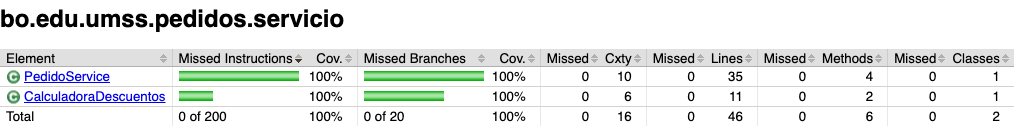
\includegraphics[width=\linewidth]{img/cobertura_resumen.png}\\[3pt]
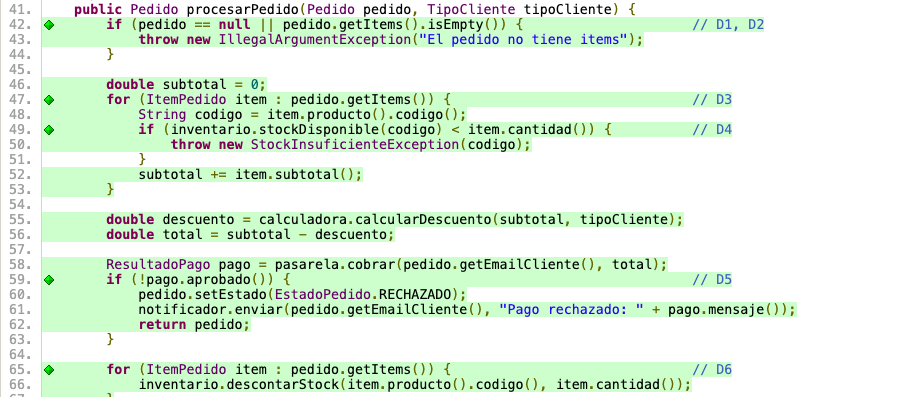
\includegraphics[width=\linewidth]{img/cobertura_codigo.png}\\[2pt]
\textcolor{verde}{$\blacklozenge$} = todas las ramas de esa decisión probadas $\Rightarrow$ \textbf{100\,\% de ramas}.
\end{columns}
\end{frame}

\begin{frame}[fragile]{Demo: ¿las pruebas detectan errores?}
\begin{columns}[T]
\column{0.52\textwidth}
\textbf{\small 1. Introducimos un error a propósito}\\[2pt]
\scriptsize En \code{PedidoService} cambiamos \code{stock < cantidad} por \code{stock <= cantidad}:
\begin{lstlisting}[style=terminal,basicstyle=\ttfamily\scriptsize\color{white}]
$ ./run.sh
|- Valor límite de stock: stock == cantidad
|  es suficiente ✘ Stock insuficiente para MON-01
|- C5: pago rechazado ✘ Stock insuficiente para P1
|- C6: pago aprobado con un item
|  ✘ Stock insuficiente para el producto P3
|- cobraAntesDeDescontarStock...() ✘ ...MOU-01
[        61 tests successful      ]
[         4 tests failed          ]
\end{lstlisting}
\scriptsize El caso de \textbf{valor límite L1} (caja negra) y los caminos C5 y C6 (caja blanca) detectan el error. Luego restauramos el código y todo vuelve a verde.
\column{0.46\textwidth}
\textbf{\small 2. Cobertura con solo caja negra}\\[3pt]
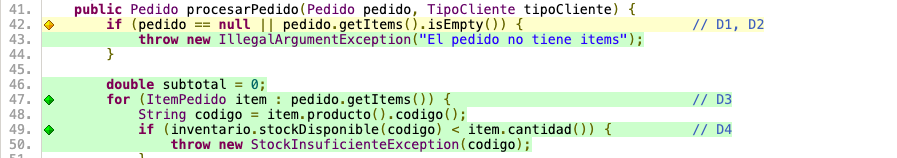
\includegraphics[width=\linewidth]{img/cobertura_cajanegra.png}\\[3pt]
\scriptsize \textcolor{anot}{$\blacklozenge$} \textbf{Rombo amarillo} en la línea 42: ``1 de 4 ramas sin probar'' (\code{pedido == null}). La SRS no lo menciona (OBS-01); solo la \textbf{caja blanca} (camino C1) lo cubre.
\begin{exampleblock}{Conclusión de la demo}
\scriptsize Las dos técnicas se \textbf{complementan}: juntas llegan al 100\,\%.
\end{exampleblock}
\end{columns}
\end{frame}

\begin{frame}{Conclusiones}
\begin{enumerate}\footnotesize\setlength{\itemsep}{1pt}
  \item Mockito aísla la clase bajo prueba: \textbf{65 pruebas en menos de 1 s} sin BD, banco ni correo.
  \item Su \textbf{arquitectura} (\code{MockHandler}, \code{MockingProgress}\ldots) explica sus reglas y sus mensajes de error.
  \item \textbf{SRS} verificable + \textbf{SDD} con interfaces inyectadas = requisitos que se pueden probar y lugares donde poner los mocks.
  \item Los casos \textbf{se diseñan paso a paso} antes de programarse, con el resultado esperado calculado a mano.
  \item Caja negra y caja blanca \textbf{se complementan}: juntas llegan al \textbf{100\,\% de ramas}.
\end{enumerate}
\begin{block}{\faSearch\ 7 principios que comprobamos}
\footnotesize \textbf{1.} Las pruebas muestran defectos, no su ausencia. \quad \textbf{2.} Probar todo es imposible: clases, límites y caminos eligen pocos casos. \quad \textbf{3.} Probar temprano ahorra: la revisión de la SRS halló 4 defectos antes de programar.
\end{block}
\begin{block}{\faSearch\ Para la auditoría de sistemas}
\footnotesize Pruebas automatizadas + trazabilidad + cobertura = \textbf{evidencia objetiva y repetible} (COBIT 2019 BAI03, ISO/IEC/IEEE 29119).
\end{block}
\end{frame}

\begin{frame}[standout]
  ¡Gracias!\\[0.4cm]
  {\normalsize Grupo 10 -- Mockito}
\end{frame}

\end{document}
